By analysis of more exclusive selection of single or multiple electroweak boson production,
it is possible with the LHC Run 1 data to isolate purely electroweak amplitudes of
increased complexity and complementary sensitivity to new physics.  The first demonstration of
this was the observation of an electroweak amplitude in $\Zzero+2$ jet production by both the
ATLAS and CMS experiments~\cite{Aad:2014dta, Khachatryan:2014dea}.

Figure~\ref{fig:ss-exclboson-z2j-sigdiagram} shows the leading order diagrams for $\Zzero+2$ jet production
from purely electroweak contributions.  It includes a vector boson fusion component similar to
VBF Higgs production, as well as electroweak bremsstrahlung amplitudes.  The different amplitudes
are strongly interfering and cannot be practically isolated from one another via kinematic selection.
In general, $\Zzero+2$ jet production is dominated by simpler Drell-Yan production accompanied by QCD bremsstrahlung,
but in certain exclusive regions of the di-jet phase space the electroweak amplitudes are dominant.

\begin{figure*}[htb] {
\centering
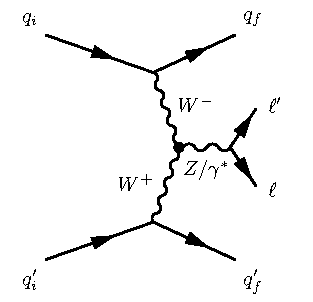
\includegraphics[width=0.315\textwidth]{figures/ss-exclboson-z2j-vbfz_diagram.pdf}
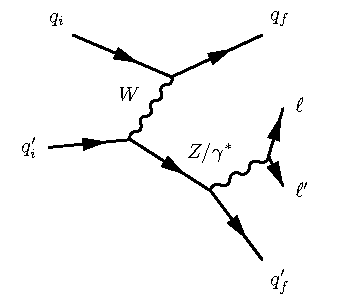
\includegraphics[width=0.35\textwidth]{figures/ss-exclboson-z2j-bckg3_diagram.pdf}
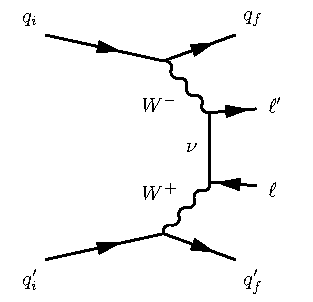
\includegraphics[width=0.315\textwidth]{figures/ss-exclboson-z2j-bckg1_diagram.pdf}
\caption{
Representative Feynman diagrams for di-lepton production in association
with two jets from purely electroweak contributions:
(left) vector boson fusion,
(middle) bremsstrahlung-like,
and (right) multiperipheral production.
\label{fig:ss-exclboson-z2j-sigdiagram}}

}
\end{figure*}


The LHC experiments have used several criteria to isolate the electroweak amplitudes.  The ATLAS analysis
defines a search region with
\begin{itemize}
    \item minimum $\pt$ of the jets (45-55 GeV) and the $\Zzero$ boson candidate (20 GeV)
    \item minimum invariant mass of the di-jet system (250 GeV)
    \item a veto on events with an additional jet in the rapidity gap between the leading two jets
    \item an upper limit (0.15) on the relative imbalance in the momenta of the four-body di-lepton and di-jet system, where
    imbalance is defined as the magnitude of the four-body $\pt$ vector sum relative to the four-body scalar sum of transverse momenta.
  \end{itemize}

CMS selects events with minimum $\pt$ of the jets (30-50 GeV), minimum invariant mass of the di-jet system (200 GeV), a maximum
magnitude of the difference between the $\Zzero$ rapidity and the avarage jet rapidity (1.2), and an upper
limit (0.14) on the relative imbalance of the three-body $\Zzero$ and di-jet system.
Additionally a multivariate discriminant is constructed which includes:
\begin{itemize}
  \item the di-jet invariant mass
  \item the sum of the magnitudes of the jet rapidities
  \item the $\Zzero$ boson rapidity
  \item the $\Zzero$ boson $\pt$
  \item ratio of the difference between the $\Zzero$ rapidity and the avarage jet rapidity to the di-jet rapidity difference
  \item a quark/gluon multivariate discriminant evaluated for the leading two jets
\end{itemize}

The ATLAS analysis extracts an electroweak signal from selected events via a maximum likelihood fit
of electroweak $\Zzero+2$ jet signal and background yields to the di-jet invariant mass distribution.
The signal template is obtained from \texttt{Sherpa} $\Zzero+2$ jet simulation and the background template also from \texttt{Sherpa},
except its shape is reweighted to obtain agreement with a separate control sample in the data.
The result of the fit is shown in Figure~\ref{fig:ss-exclboson-z2j-8tev}.  An excess of data over background begins to be seen
near 1000 GeV in di-jet mass, increasing in significance for higher di-jet masses, totalling close to 1700 events with a statistical
significance greater than 5$\sigma$.   A high-purity fiducial cross section region is defined for events in the search
region above 1000 GeV in di-jet mass, where the signal yield is obtained from integrating the signal component of the likelihood fit.
The resulting electroweak cross section is
$$\sigma_{EW} (m_{jj} > 1 \TeV) = 10.7 \pm 0.9 \rm{(stat)} \pm 1.9 \rm{(syst)} \pm 0.3 \rm{(lumi)} \rm{\,fb}$$,
in agreement with the \texttt{Powheg} prediction of $9.4\pm0.3 \rm{\,fb}$.  The systematic uncertainty is predominantly from
control sample statistics for background reweighting, the simulation modelling of signal and background,
and estimates of the effect of neglecting signal-background interference.

\begin{figure}[p]
    \centering
    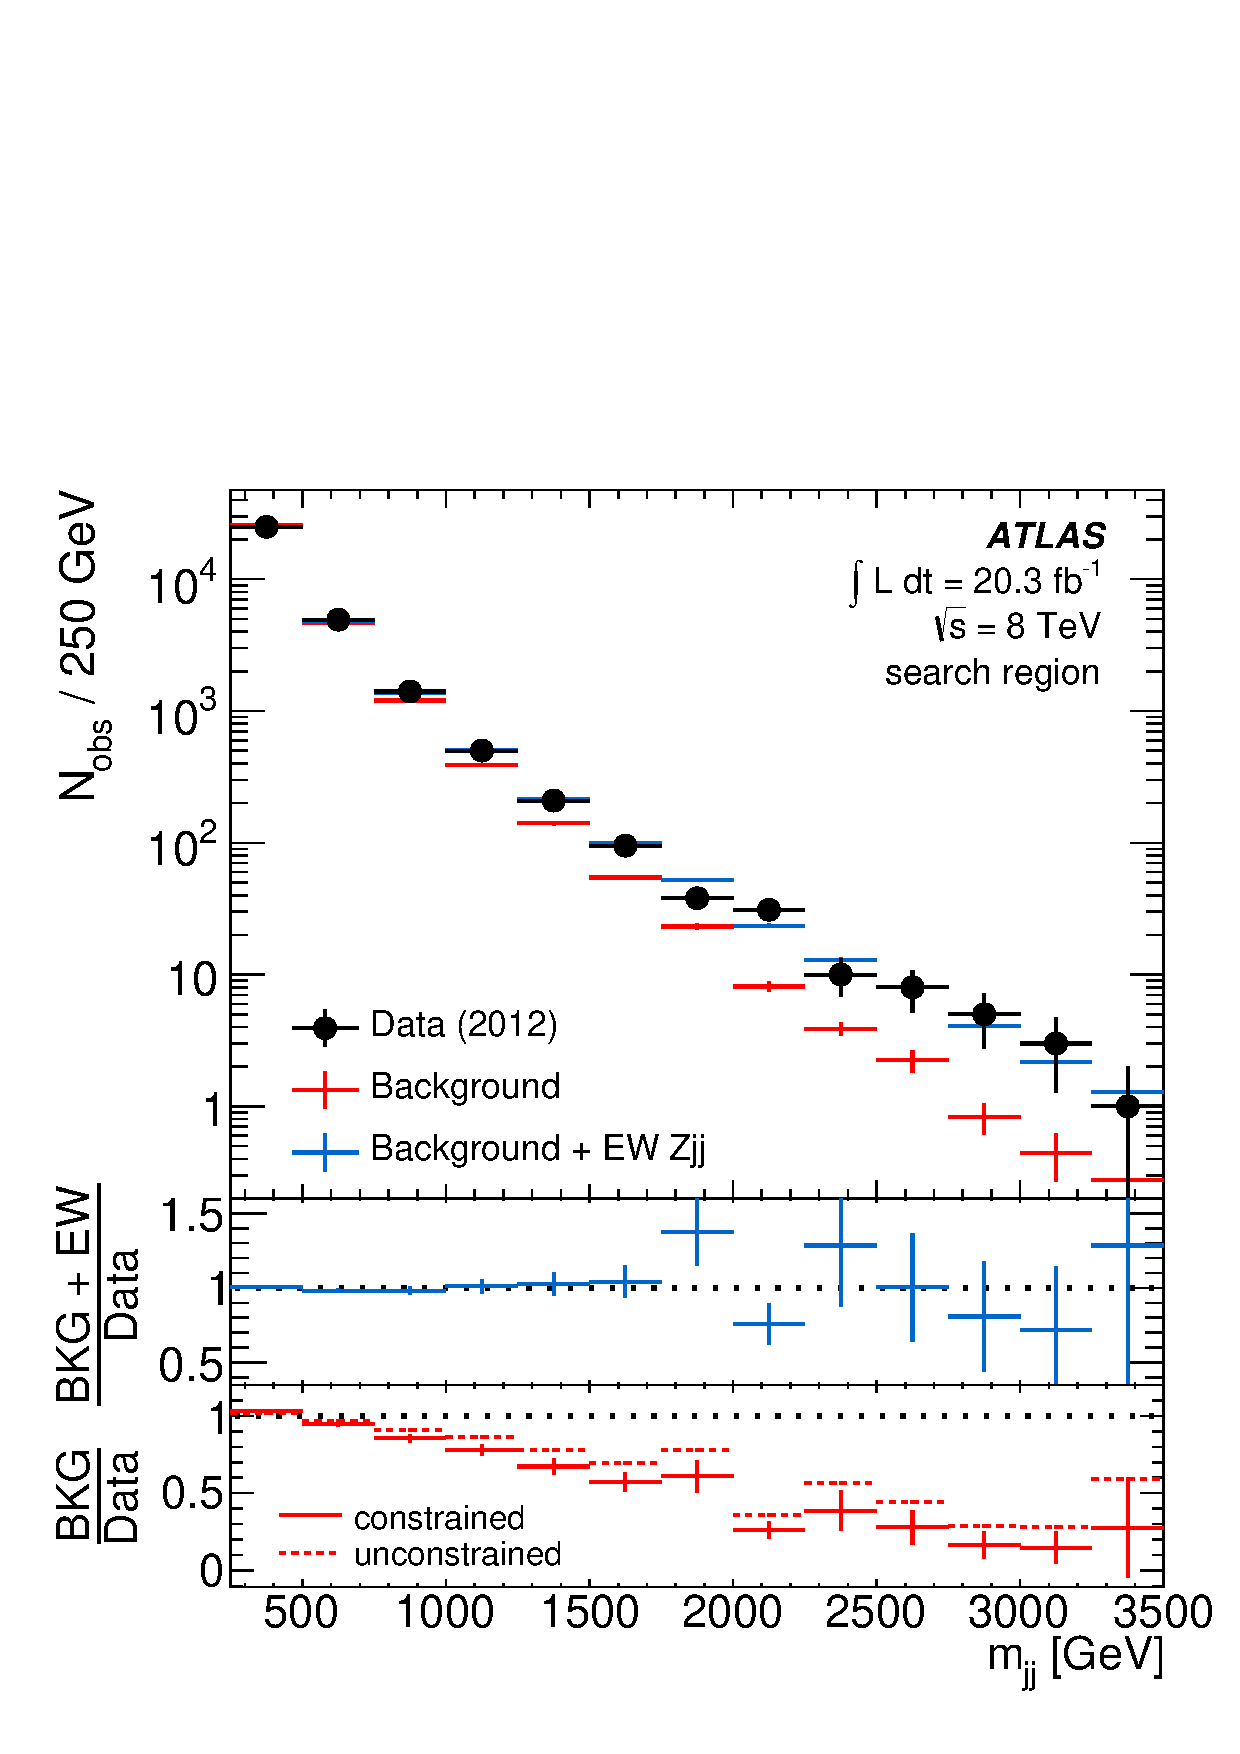
\includegraphics[width=0.45\textwidth]{figures/ss-exclboson-z2j-atlas8tev.pdf}
    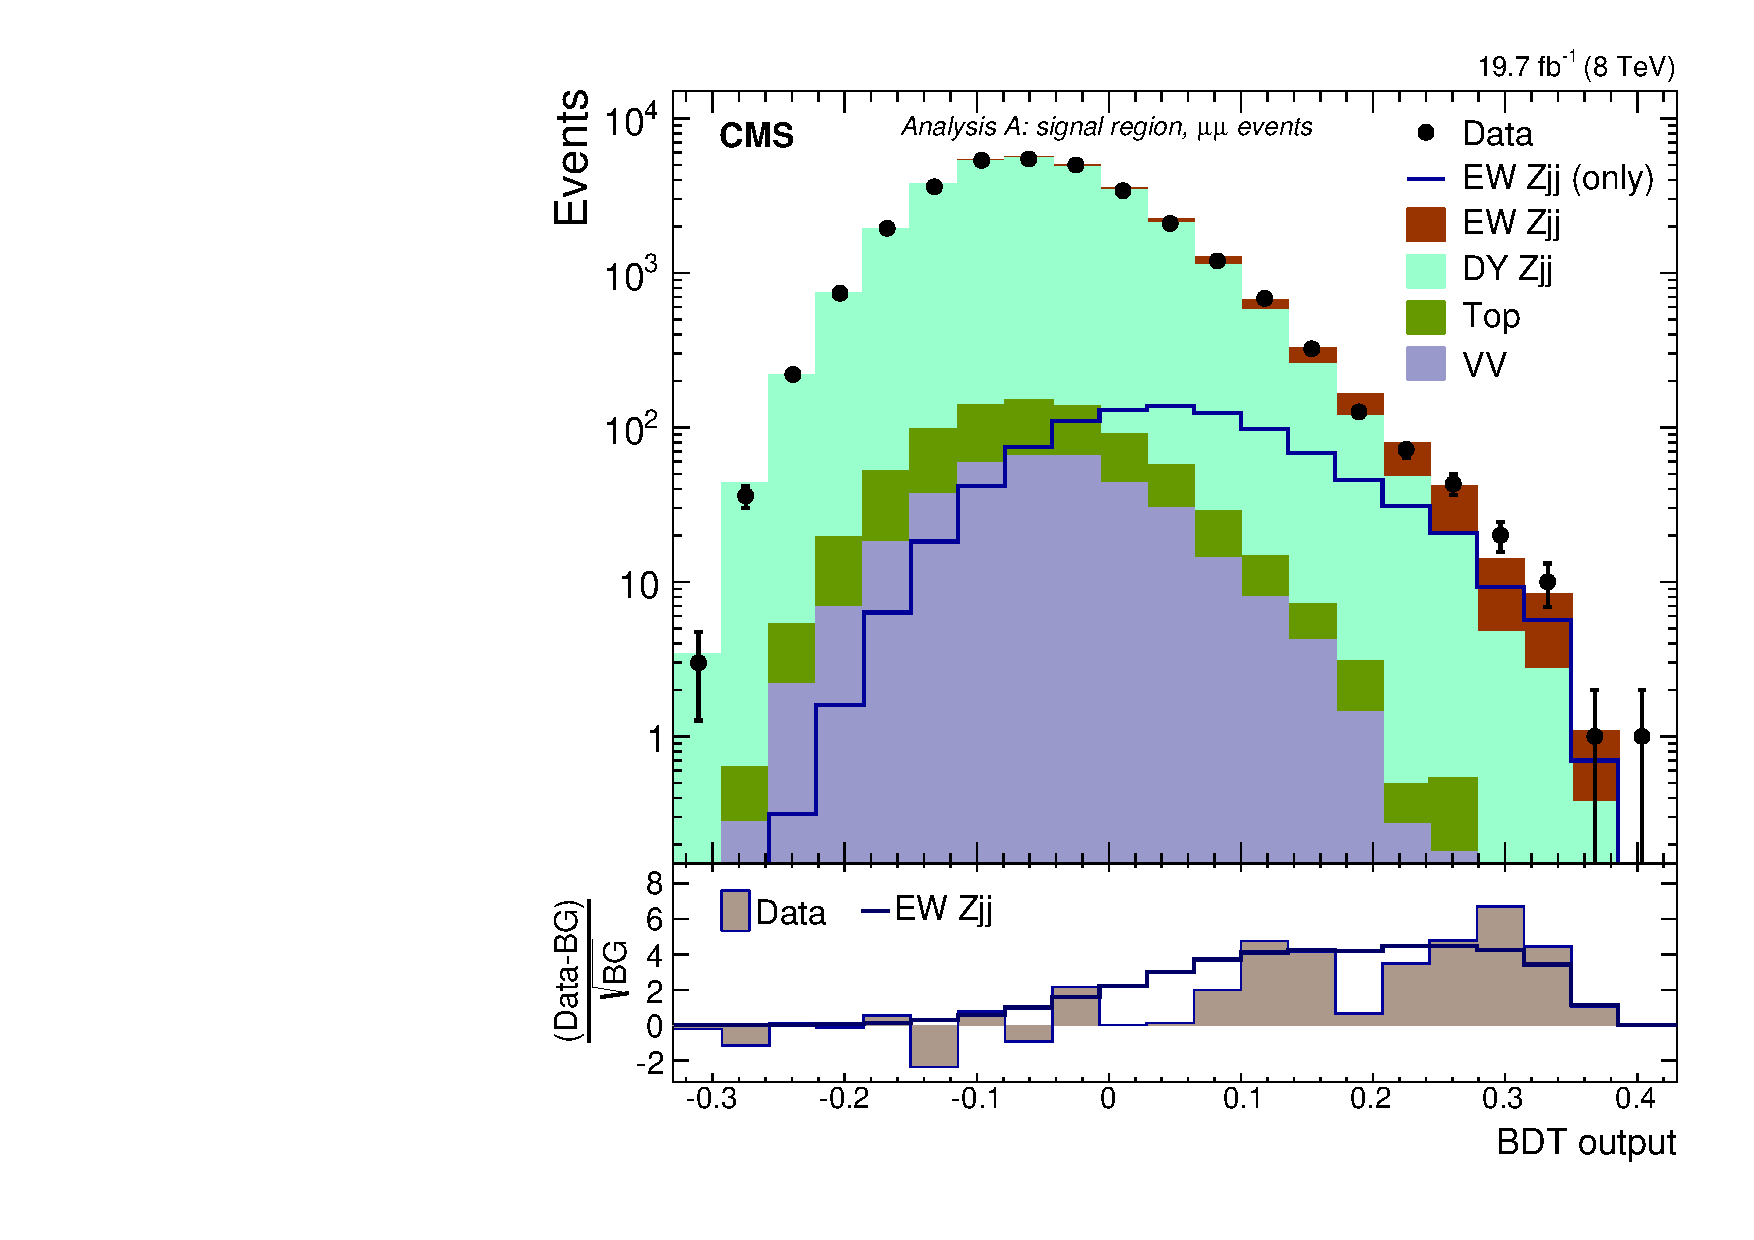
\includegraphics[width=0.45\textwidth]{figures/ss-exclboson-z2j-cms8tev.pdf}
    \caption{Evidence of observation of an electroweak amplitude in $\Zzero+2$ jet production.
    Left:  The invariant mass distribution of di-jets in $\Zzero+2$ jet events selected
     from a signal region by ATLAS~\cite{Aad:2014dta}.
    Right:  The BDT distribution of $\Zzero+2$ jet events selected from a signal region
    by CMS in the di-muon channel~\cite{Khachatryan:2014dea}.}
    \label{fig:ss-exclboson-z2j-8tev}
\end{figure}

Similarly, CMS extracts an electroweak signal via a likelihood fit to the kinematic multivariate discriminant.  The signal and background
templates are obtained from \texttt{MadGraph}, 
and an interference term is introduced proportional to the square root of the signal strength.
The background shape is not reweighted but comparisons between data and simulation control samples bound shape uncertainties.  A signal significance
greater then 5$\sigma$ is observed, corresponding to a signal yield close to 1600 events, as shown in Figure.~\ref{fig:ss-exclboson-z2j-8tev}.
For a fiducial cross section corresponding to all selected events, they obtain
$$\sigma_{EW} = 174 \pm 15 \rm{(stat)} \pm 40 \rm{(syst)} \rm{\,fb}$$,
in agreement with the \texttt{MadGraph} prediction of $208 \pm
18 \rm{\,fb}$.  Total systematic uncertainties types and sizes are
similar to that of ATLAS. In both experiments the systematic
uncertainty associated with interference effects is an estimate of the
whole difference between including or excluding its contribution, and
is estimated at 17\% and 6\% from CMS and ATLAS, respectively.
